\pdfoutput=1

\documentclass[11pt,a4paper]{article}
\renewcommand\thesection{\Alph{section}}
\renewcommand\thesubsection{\arabic{subsection}}
\renewcommand\thesubsubsection{\thesubsection.\arabic{subsubsection}}
\usepackage[a4paper, total={6.5in, 10in}]{geometry}
\usepackage{setspace}
\doublespacing

\usepackage{lastpage}
\usepackage{fancyhdr}
\pagestyle{fancy}
\fancyhf{}
\fancyhead[L]{Mael GOODALL Léo STEINBACH\hfill\leftmark\hfill\today}
\fancyfoot[C]{p. \thepage/\pageref{LastPage}}
\renewcommand{\footrulewidth}{0.3pt}
\setlength{\headheight}{14.5pt}

\usepackage[bf,raggedright]{titlesec}
\titlespacing*{\section}{-40pt}{5.5ex plus 1ex minus .2ex}{1.5ex plus .2ex}
\titlespacing*{\subsection}{-40pt}{3.25ex plus 1ex minus .2ex}{1.5ex plus .2ex}
\titlespacing*{\subsubsection}{-30pt}{3.25ex plus 1ex minus .2ex}{0.5ex plus .2ex}

    \title{TP filtrage numérique}

\author{Mael GOODALL Léo STEINBACH}
\date{\today}
\usepackage{graphicx}
\graphicspath{{images/}}
\usepackage{mathrsfs}
\usepackage{amsfonts}
\usepackage{amsmath}
\usepackage{amssymb}


\newcommand{\diff}{\mathop{}\mathopen{}\mathrm{d}}
\newcommand{\parenth}[1]{\left( #1 \right)}
\newcommand{\df}[2][]{\frac{\diff #1}{\diff #2}}



\begin{document}
\newgeometry{top=-0.2in}
\maketitle
\thispagestyle{fancy}
\tableofcontents
\restoregeometry

    \subsection{}
        \subsubsection{}
            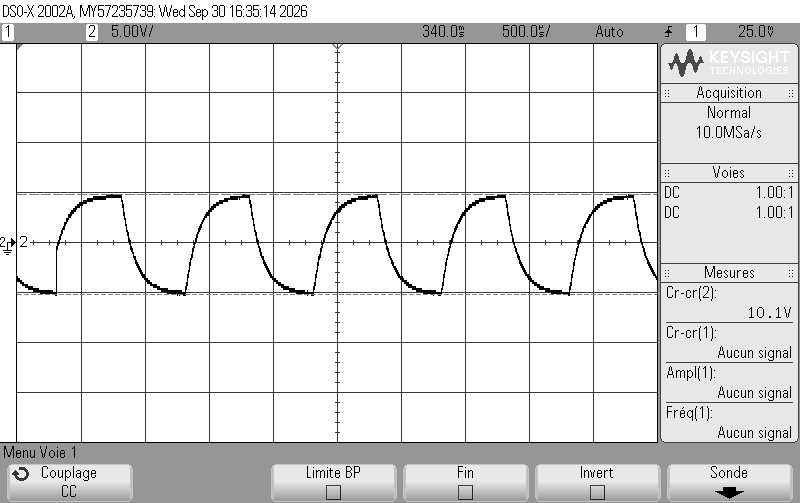
\includegraphics[scale=0.6]{scope_3.png}\\
            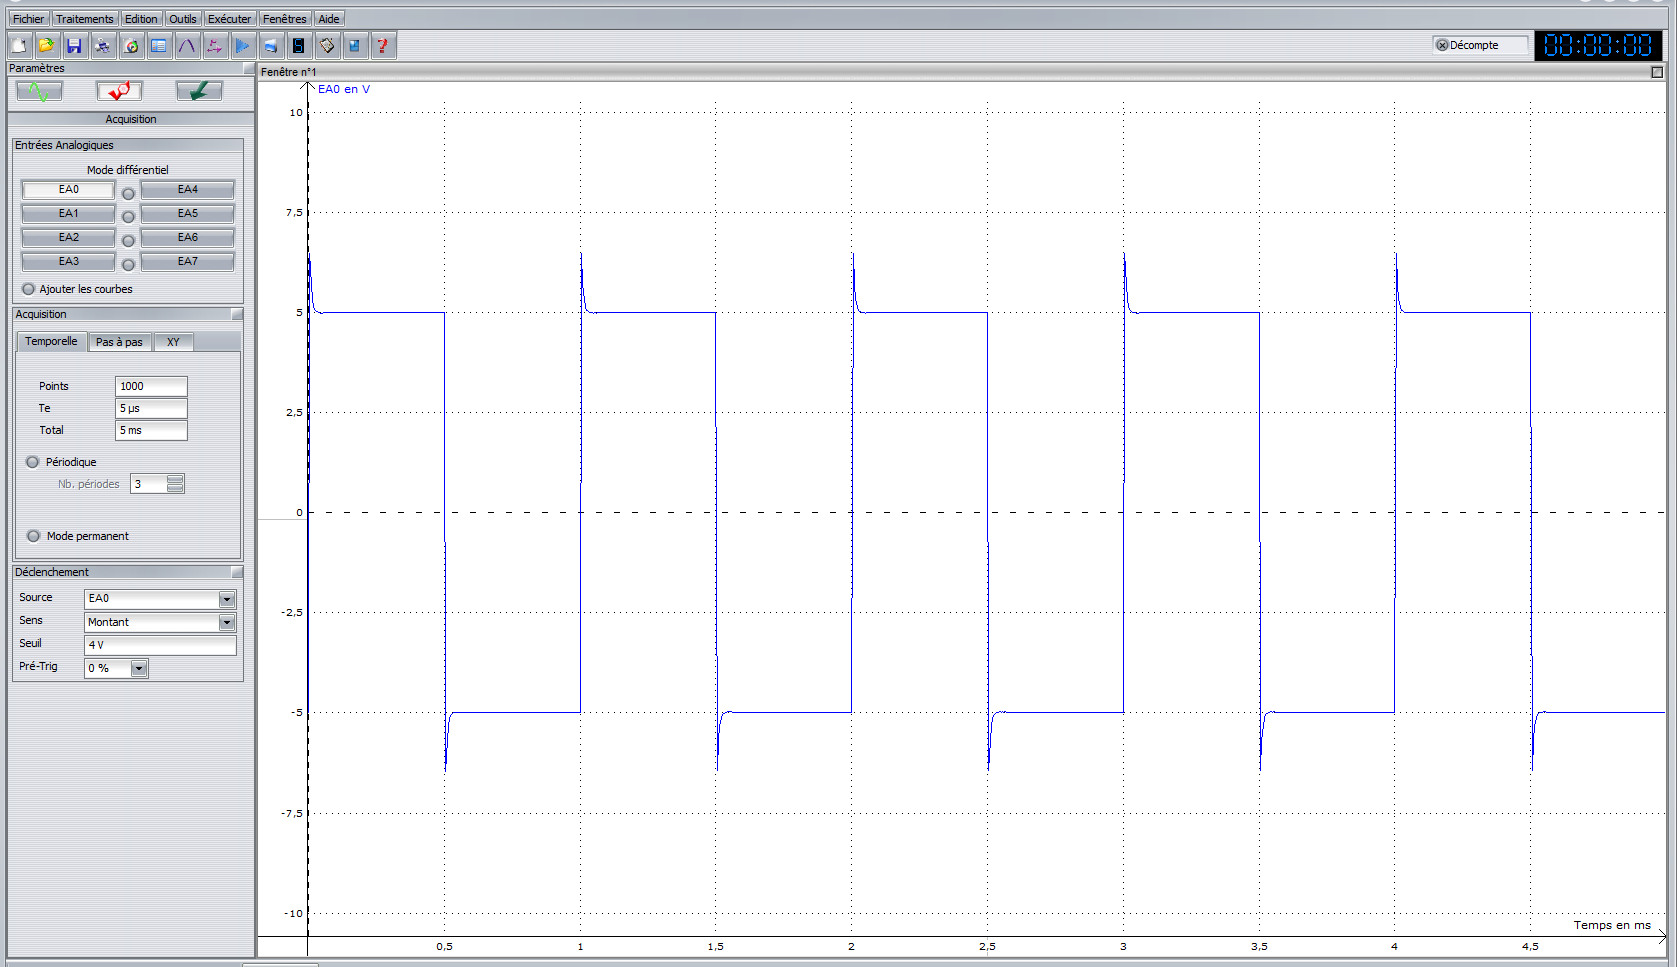
\includegraphics[scale=0.4]{Signal1.2.png}\\
            Le signal convient car on observe distinctement plusieurs pèriodes.
        \subsubsection{}
            $H_0(\omega)=\frac{1}{1+j\frac{\omega}{omega_0}}$ donc :
            \[\df{y}{t}+\frac{y}{\tau}=\frac{x}{\tau}\]

    \subsection{}
        \subsubsection{}\label{2.1}
            La durée entre deux échantillons succéssifs est : $T_e=5\mu s$

            On peut prendre l'aproximation : $\df{y(t)}{t}= \frac{y_{n+1}-y_n}{T_e}$

            Donc : $\frac{y_{n}-y_{n-1}}{T_e} + \frac{y_n}{\tau} = \frac{x_n}{\tau}$

            Soit : $y_{n} = \frac{1}{1+\frac{\tau}{T_e}}\parenth{y_{n-1}\frac{\tau}{T_e}+x_n}$
            
            D'où : $\alpha = \frac{\tau}{T_e} = 20$

        \subsubsection{}
            On mesure la tension aux bornes du condensateur (déchargé) donc $y_0 = 0$V

            La première ligne permet d'initialiser le tableau des valeurs de $y_n$ 
            la deuxième ligne permet de calculer récursivement les valeurs de $y_n$ grace à la formule obtenu en \ref{2.1}.\\
            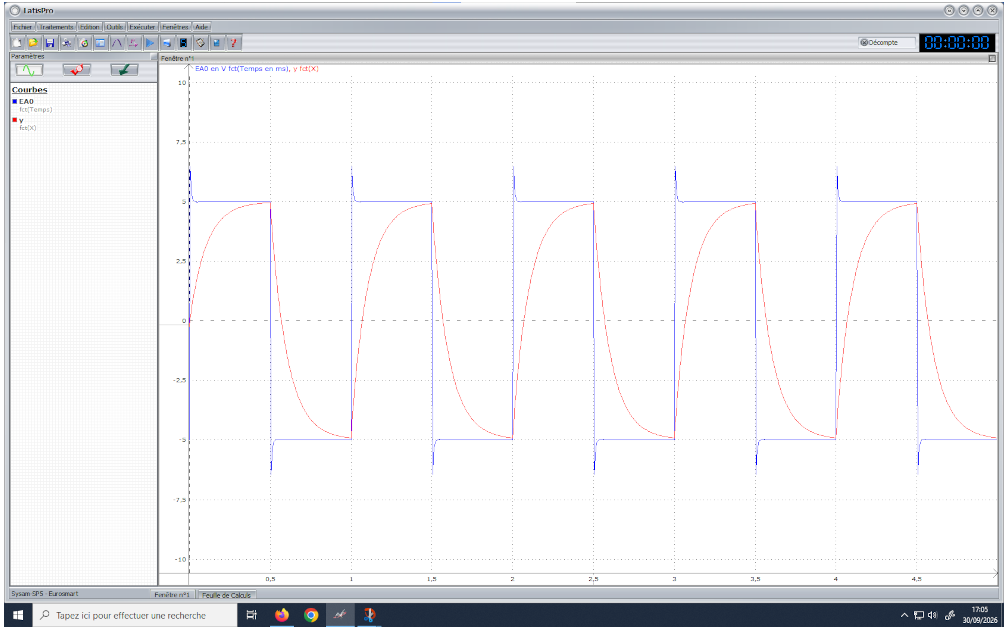
\includegraphics[scale=0.6]{2.2.png}

        \subsubsection{}
            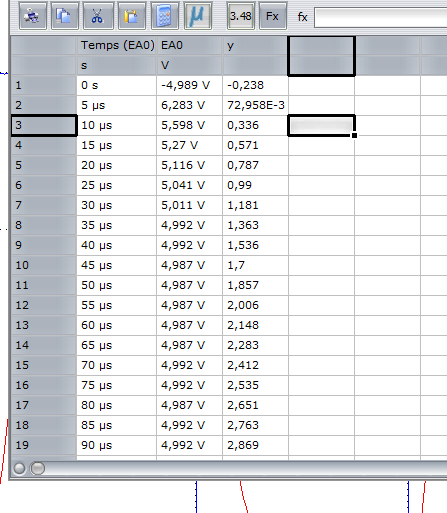
\includegraphics[scale=0.8]{Tableur.png}

        \subsubsection{}
            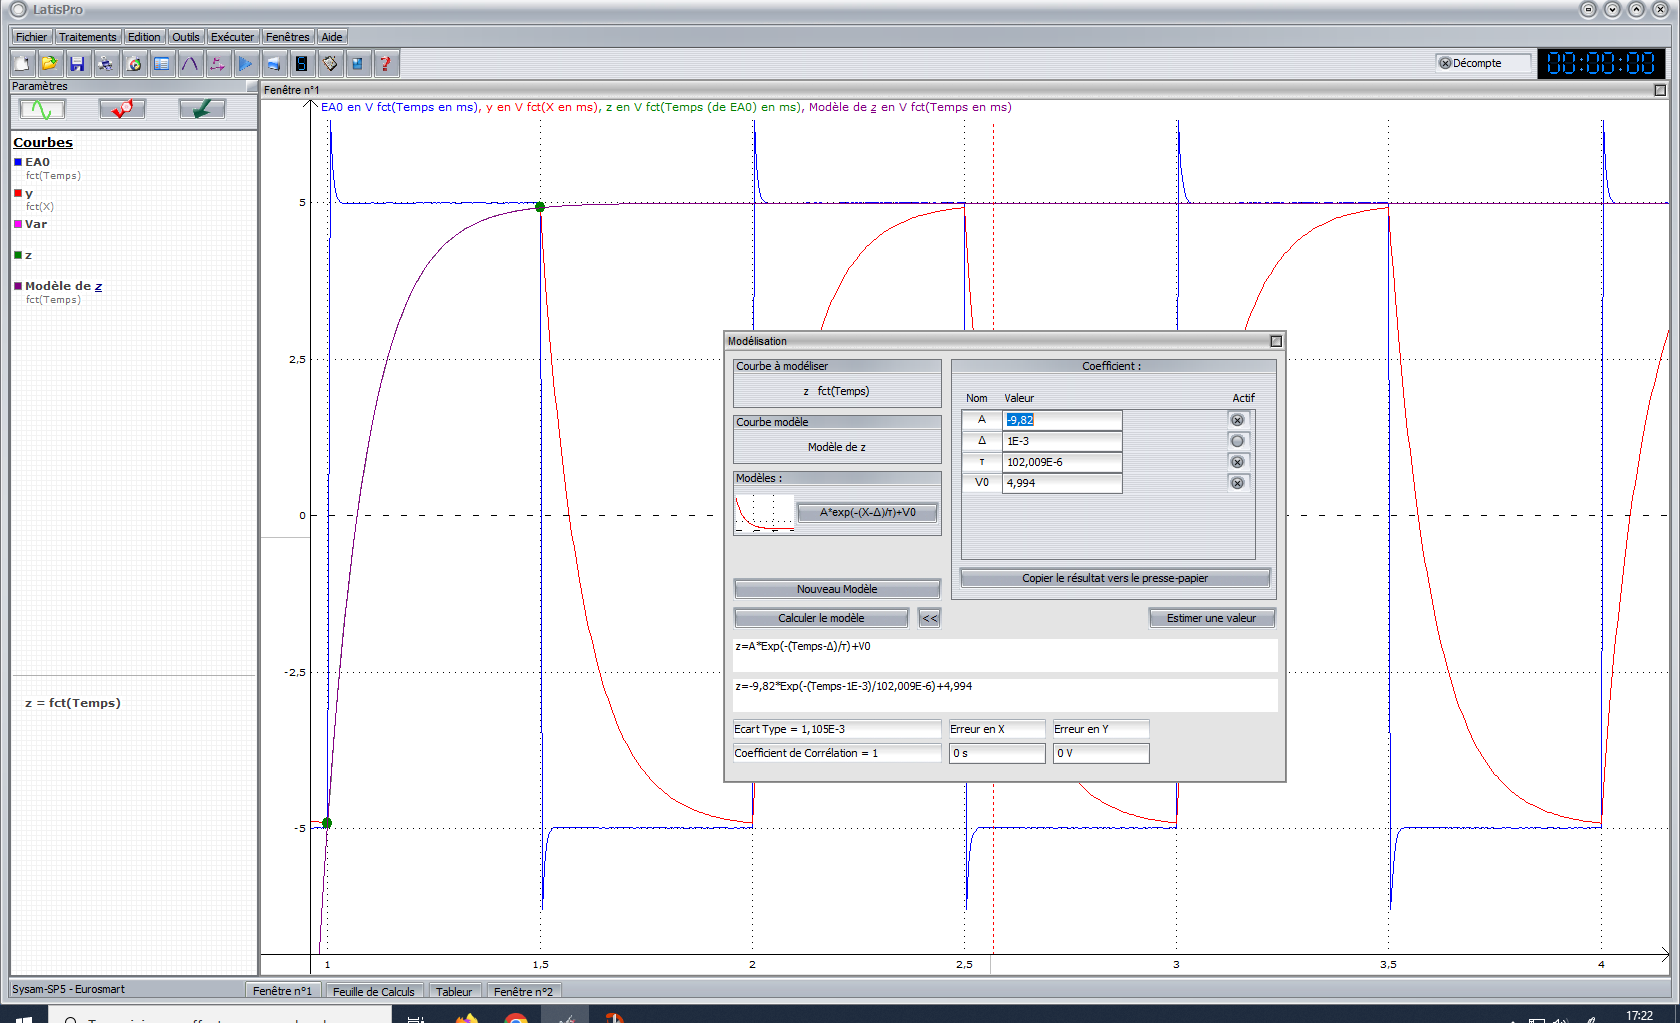
\includegraphics[scale=0.4]{Z.png}\\
            On a $\Delta=\Delta_{th}$ et $V_0=V_{0,th}$ à $0.1\%$ près et $\tau=\tau_{th}$ à $2\%$ près
        
        \subsubsection{}
            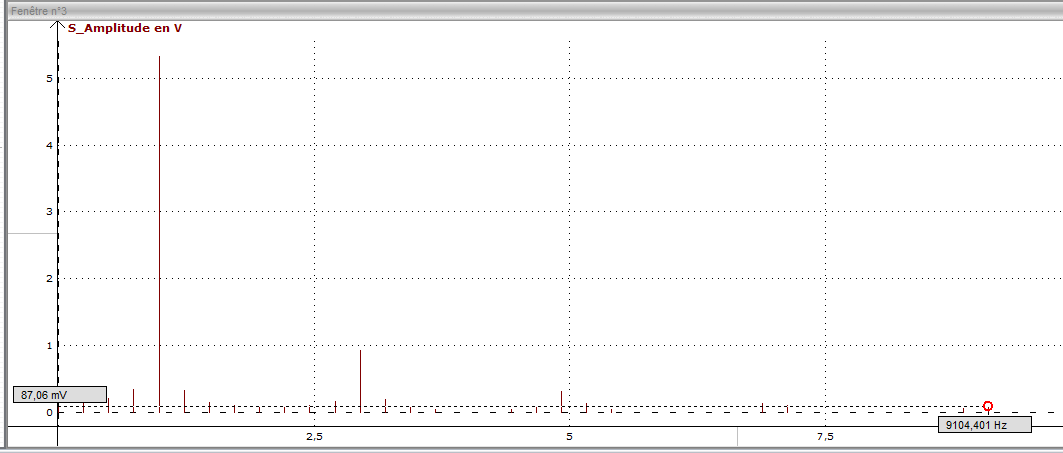
\includegraphics[scale=0.6]{Ordre9.png}%montage 


\end{document}
